\documentclass{beamer}
\mode<presentation>

\usepackage{header_footer}
\usepackage{pgfpages}
\usepackage{bbm}
\usepackage{amsmath}
\usepackage{amssymb} 
\usepackage{amsthm}
\usepackage{epsfig}
\usepackage{natbib} 
\usepackage{apalike}
\usepackage{floatrow}
\usepackage{wasysym}
\usepackage[absolute,overlay]{textpos}
\usepackage[version=4]{mhchem}
\usepackage[long,nodayofweek,level,12hr]{datetime}
\makeatletter 
\def\newblock{\beamer@newblock}
\makeatother
\usepackage{color}
\usepackage{graphicx}
\usepackage{epstopdf}

\definecolor{CASblue}{rgb}{0.611764706, 0.76862745098, 0.95294117647}
\setbeamercolor{frametitle}{fg=CASblue}
\setbeamerfont{frametitle}{series=\bfseries}

\newcommand{\tit}{Timing Side-Channel Attack}
\newcommand{\subt}{Using linear correlation to reveal secrets}
\newcommand{\auth}{A. Anselmo, S.A. Chiaberto, F. Chiatante, G. Roggero}
\newcommand{\inst}{EURECOM}
\newcommand{\supervisor}{Prof. Renaud Pacalet}
\newdate{dat}{21}{06}{2019}
\newcommand{\ddat}{\displaydate{dat}}
\newcommand{\rd}{\quad \ddat \quad \tit}

\setbeamercolor{item}{fg=black} 
\setbeamertemplate{itemize items}[circle] 
\setbeamertemplate{itemize subitem}[ball] 
\setbeamertemplate{itemize subsubitem}[triangle]

\beamertemplatenavigationsymbolsempty 

\title{\tit }
\subtitle{\subt}
\author{\auth }
\institute{\inst }
\date{\ddat}

\begin{document}
\newcommand{\presentationtitle}[5]{
    \begin{frame}[plain]
    \myheader
    \begin{center}
    \textcolor{black} {\sc\huge #1} \\[0.2cm]
    \textcolor{black} {\small #2} \\[0.9cm]
    \textcolor{black} {\bf\small #3} \\[0.5cm]
    \end{center}
    \textcolor{black}{\small Supervisor: \textit{#5}}
    \hfill
    \textcolor{black} {\small #4} \\[0.4cm]
    \vfill
    \myfooter
    \end{frame}
}

\presentationtitle{\tit}{\subt}{\auth}{\ddat}{\supervisor}
\begin{frame}
\frametitle{Outline} 
\setbeamercolor{section in toc}{fg=black}
\setbeamercolor{subsection in toc}{fg=gray}
\tableofcontents
\end{frame}

\section{Introduction}

\begin{frame}
\frametitle{Introduction}

\begin{itemize}
\item in several algorithms used for security purposes some optimizations are introduced
\item these optimizations lead to a linear dependency between time and the data encrypted
\item knowing information regarding the time-data pair, it is possible to find a correlation
\item this correlation can be used to unveal part of the secret
\end{itemize}
\end{frame}

\subsection{Hypothesis}
\begin{frame}{Hypothesis}
    \begin{block}{Tools needed}
        In order to successfully extract the secret through the correlation, we have to make a list of assumptions:
        \begin{itemize}
            \item timing for a sufficiently large number of cyphertexts is known
            \item cyphertexts are known
            \item secret is the same for all cyphertexts
            \item the HW/SW implementation is known to the attacker
            \item a timing model can be built
        \end{itemize}
    \end{block}
\end{frame}

\subsection{Library development}
\begin{frame}{From the very beginning}
	\begin{block}{BIGINT required}
		In order to operate with large integers, we decided to develop our own library of functions to operate over integers of arbitrary length, in particular with the following elementary instructions:
		\begin{itemize}
			\item addition and subtraction
			\item multiplication
			\item bitwise operation, such as \texttt{AND, OR, XOR, NOT}
			\item logical comparison
		\end{itemize}
	\end{block}
\end{frame}


\section{Attack}
\subsection{Algorithm}
\begin{frame}[fragile]
	\frametitle{Finding correlations}
	\begin{block}{PCC: our game changer}
		In order to find the linerar contribution of each sample in the overall time, we have used the \textit{Pearson Correlation Coefficient} as an estimator. It has proved to be really effective for our needs, working on the realizations of a random variable.
	\end{block}
	\begin{center}
		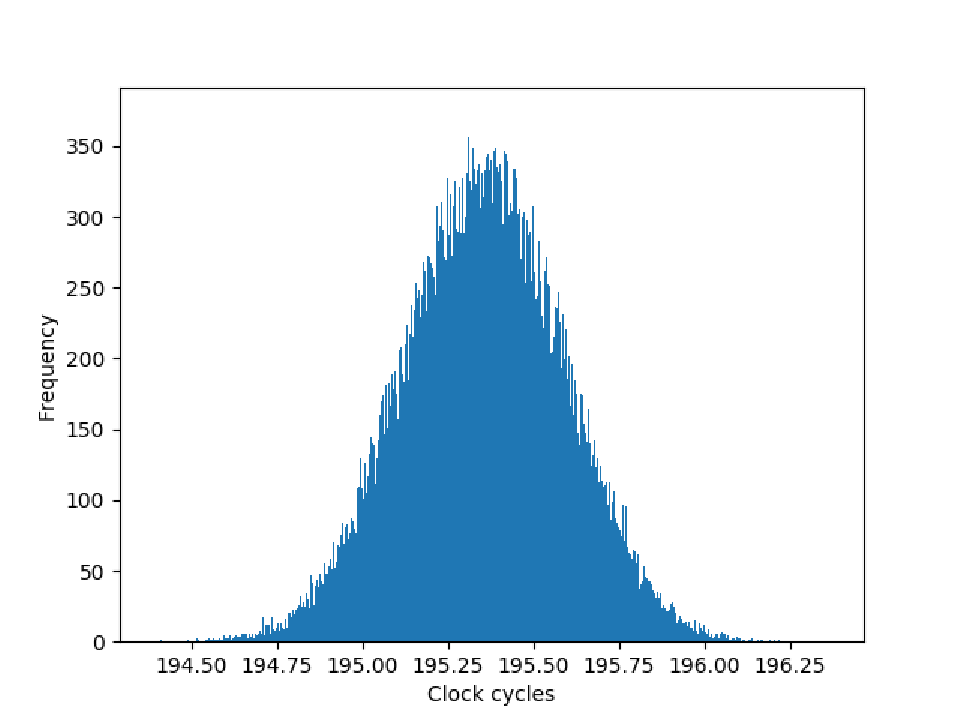
\includegraphics[width=6cm]{./graphics/rand_distr}
	\end{center}
\end{frame}


\section{Counter}

\begin{frame}[fragile]
\frametitle{Titlepage settings}
\begin{itemize}
\item by changing settings in \begin{verbatim} header_footer.sty \end{verbatim} you can choose whether and where you want a second logo to be positioned on the titlepage:
\begin{itemize}
\item small logo can be placed on the bottom right
\item big logo can be placed on the top right
\end{itemize}
\item spaces and graphics dimensions will have to be adjusted depending on your logo
\end{itemize}
\end{frame}

\begin{frame}[fragile]
\frametitle{Outline}
\begin{itemize}
\item divide the presentation, using the command {\tt section} 
(as it is usually done in \LaTeX) 
\item other divisions, just as chapter or part are not supported
\item the sections are are listed on the top of each slide, the section the 
recent slide belongs to is highlighted
\item you can automatically receive an outline out of this section by the command
\begin{verbatim}
\tableofcontents
\end{verbatim}
\end{itemize}
\end{frame}


\section{Possibilities}

\begin{frame}
\frametitle{Itemize}
\begin{itemize}
\item black circle is the default; other possibilities are:
\begin{itemize}
\item ball
\begin{itemize}
\item triangle
\end{itemize}
\end{itemize}
\item the color of the items can also be changed
\item all this settings have to be done in the preamble of the {\tt presentation.tex} file
\end{itemize}
\end{frame}

\begin{frame}
\frametitle{Overlays}
\begin{itemize}
\onslide+<2-> {\item its possible to build slides succesively} 
\onslide+<3-> {\item to do so use the command {\tt onslide} }
\onslide+<4-> {\item other useful commands are {\tt uncover} and {\tt only} }
\onslide+<5-> {\item this works also very nice to ''develop'' formulas: }
\[
\onslide+<6-> {f (x \mid \mu, \sigma^2) ~=~ } 
\onslide+<7-> { \frac 1 {\sigma\sqrt{2\pi}} }
\onslide+<8-> { \cdot \exp\left\{ }
\onslide+<9-> { -\frac {(x-\mu)^2} {2\sigma^2} }
\onslide+<8-> { \right\} }
\]

\end{itemize}
\end{frame}


\section{Graphics}

\begin{frame}[fragile]
\frametitle{Pimp up your presentation}
\begin{itemize}
\item an easy way to include pictures is by using
\begin{verbatim}
\includegraphics[width=...,height=...]{file}
\end{verbatim}
\item in connection with {\tt pdflatex} this supports a wider range of graphic formats, including GIF, PNG, JPG \\[0.3cm]
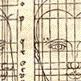
\includegraphics[width=2cm,height=2cm]{./graphics/FF4.jpg}
\end{itemize}
\end{frame}

\section{Useful Hints}

\begin{frame}[fragile]
\frametitle{Useful hints}
\begin{itemize}
\item if you use a verbatim environment on a slide, declare that slide {\tt fragile}:
\begin{verbatim}
\begin{frame}[fragile]
\end{verbatim}
\item bibliography actually works as usual, just keep in mind that not all bibliography styles are supported by the {\it beamer}
      package, maybe you have to include some other packages to get your preferred style working  
\end{itemize}
\end{frame}

\nocite{*}

\section{Countermeasures}
\begin{frame}{Possible solution}
    \begin{block}{Blinding}
		The proposed countermeasure is the one given in \cite{kocher1996timing}.
		It consists in blinding the message before the encryption using a couple of values $v_f, v_i$ chosen in such a way that:
		\begin{equation*}
			v_i^e \cdot v_f mod\: N = 1
		\end{equation*}
    \end{block}
\end{frame}

\begin{frame}[allowframebreaks]
	\frametitle{References}
%\Large{References} \\[0.5cm]
	\footnotesize
	\bibliographystyle{apalike}
	\bibliography{./bibliography/LaTeX}
\end{frame} 

\end{document}